\chapter{Choix des données et munging}

Tout d'abord \textbf{seulement les notes de 4 et 5 sont conservées}. En effet le but est de connaitre les préférences des utilisateurs, pas les genres de films qu'ils notent.
\bigskip
\\Ensuite il s'agit de choisir les variables à étudier. Pour les utilisateurs sont gardés:
\begin{itemize}
  \item L'âge
  \item Le sexe
  \item L'occupation professionnelle
  \item Le code ZIP
\end{itemize}
Le munging est comme suit: l'âge devient une variable qualitative en ne conservant que le premier chiffre de l'âge (35 devient 30, 42 devient 40 etc.). Puisque le sexe est variable binaire, les utilisateurs sont scindés en deux groupes pendant les AFCs, en effet cela permet de rajouter une variable aux AFC qui étudient les relations entre deux variables. L'occupation professionnelle reste intacte. Chaque code ZIP est associé à l'état américain qui lui est propre ou bien à la valeur \emph{Other} pour les codes éronnés et les pays étrangers aux Etats-Unis.
\bigskip
\\Pour les films sont gardés:
\begin{itemize}
  \item La date de sortie
  \item Le(s) genre(s)
\end{itemize}
Pour le munging la décennie de sortie du film est extraite. Un film peut avoir plusieurs genres et donc un choix s'impose. Pour les AFCs les tableaux de contingence prennent en compte le fait qu'aimer un film qui a deux genres équivaut à aimer un film du premier genre \underline{et} un autre film d'un autre genre. Pour l'ACM on procède de la même façon.
\bigskip
\\Tout le munging est effectué en \emph{Python} avec l'aide du module \emph{pandas}. Une jointure est effectuée sur les trois fichiers csv fournis. Des tableaux de contingence pour les AFCs sont sauvegardés sous format csv, les analyses sont effectués avec \emph{R}. Les données sont filtrées comme indiqué précédemment. Les mêmes tableaux de contingence sont construits pour les hommes et les femmes. L'API \emph{api.zippopotam.us} est utilisée pour convetir les codes ZIP en états américains qui sont ensuite filtrée selon la carte suivante.
\begin{figure}[htd]
\centering
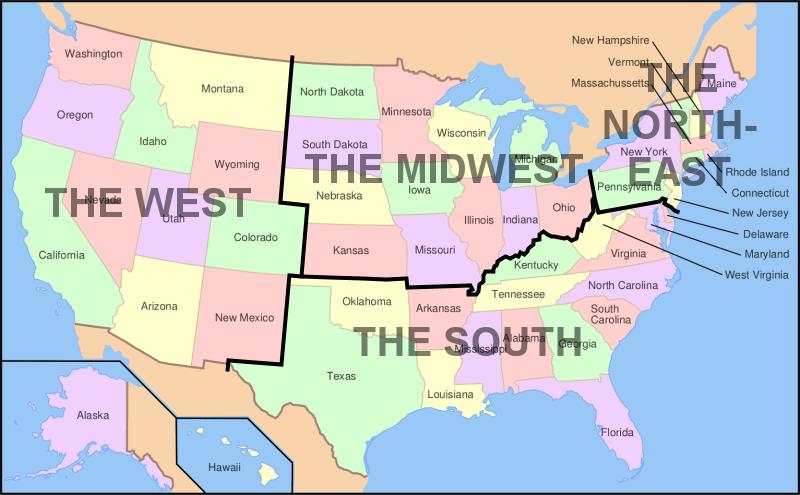
\includegraphics[scale=0.5]{./images/usRegions}
\caption{Régions des Etats-Unis}
\end{figure}
Toutes les données sont sauvegardées comme suit:
\begin{itemize}
  \item Un fichier csv contenant toutes les données.
  \item Une fichier csv contenant les données utiles à l'ACM.
  \item Une base de donnée MongoDB contenant toutes les données.
\end{itemize}
Le premier fichier sert à construire les tableaux de contingence pour produire les AFCs. Le deuxième diffère du premier car il ne contient pas toutes les données, de plus les genres de films sont séparés (par exemple un film ayant trois genres devient trois lignes). La base MongoDB est utilisée pour deux raisons. D'une part la création des tableaux de contingence pour les AFCs relatifs aux genres des films est très rapide, en effet le module \emph{pymongo} renvoit un curseur Python, un type de données natif qui permet d'itérer plus rapidement que sur un tableau de données. D'autre part une base de données peut servir dans le cas de l'étude d'une sous-population particulière d'une grande population, en effet les temps de calculs pourraient être long si on élargit notre étude au jeu de données de 10 millions de lignes de MovieLens. De la même façon calculer l'ACM avec \emph{R} pourra se révéler hardu sur le jeu de données de 10 millions de ligne, pour cela il serait envisageable d'utiliser \emph{Julia}, notamment grâce à https://github.com/MaxHalford/MultivariateStats.jl. 